\section{Detailed Architecture}
\label{DetailedArchitecture}
In this Section we introduce the tool we use to realize the chosen methodological approach. In addition, we describe the constraints under which we carry out the transformation, such as the use of a BPEL subset and the specification of a workflow pattern.
Later in this Section, we introduce the design ideas of our transformation and the general architecture we adopted.\\

FIXME: TO REMOVE LATER
\begin{itemize}
 \item *The M2T tool we use (Acceleo)
 %\item The additional components (A WebService)
\end{itemize}

The main points and some more decision we have to take over:
\begin{itemize}
  \item * We identify the subset of BPEL instructions suitable for a proof of concept of the transformation. 
  \subitem * Select a BPEL meta-model that covers the chosen subset of instructions.
  \subitem * Individuate a BPEL workflow pattern to work on 
 
 \item * Provide a transformation strategy from the BPEL constructs to Java concepts
    \subitem * the usage of the wsdl-to-java routine to create the tree of messages types
    \subitem * all written
 \item * Design the architectural structure of the output Java application.
 \item * Define the essential skeleton of Java classes necessary to create a runnable BPEL process
 \item * In the templates, describe how to use and where the dynamic information taken from the BPEL input model has to be placed.
 \item Plan where and how, in the architecture, the developer intervention has to take place.
 \item \textbf{Issues encountered and proposed solutions  ?}
\end{itemize} 
 
 To mention later: \\
 StubPartnerLinks, code to be input by the user, static code, the problem with the WSDL file

% \begin{itemize}
%  \item Metamodel 
%  \item Skeleton 
%  \item Generator 
% \end{itemize}

%//////////////////////////////////////////////////////////
\subsection{The M2T Generator}
To implement our model-to-text methodology we make use of the Acceleo generator. As described in Section \ref{acceleo}, Acceleo takes as input a model in any kind of modeling language followed by its meta-model descriptor, and a series of templates defining the structure of the output text to create.
With a well defined Acceleo transformations, we can obtain runnable 
Acceleo provides us the opportunity to both navigate the parameterized input model and to plan the design of the Java templates in order not to have redundant code.
%//////////////////////////////////////////////////////////
\subsection{The BPEL subset of instructions}
\label{Sec:BPELsubset}
The BPEL standard (see Section \ref{BPEL} for more details) has a wide variety of elements and instructions aimed at managing the possible workflow patterns obtainable during a services orchestration. Moreover, BPEL does not restrict the number of services that can participate to the orchestration neither the type and the quantity of interactions among them.
For these reason, we focus our attention on a subset of the whole BPEL language, both to restrain the complexity and to fit the time frame of the project.
\subsubsection{The activities subset}
We decided to restrict the BPEL activities to a subset containing the following constructs divided in four groups:
\begin{center}
\begin{supertabular}{p{0.4\textwidth}p{0.4\textwidth}}

1. Basic activities: 			& 2. Structured activities:		\\
\begin{itemize}
	\item \verb|<invoke>|
	\item \verb|<receive>|
	\item \verb|<reply>|
	\item \verb|<assign>|
	\end{itemize} 			&

					    \begin{itemize}
					      \item \verb|<sequence>|
					     \end{itemize}			\\
					     
3. Elementary operations: 		& 4. Static descriptive elements:	\\					
\begin{itemize}
	\item \verb|<copy>|
	\item \verb|<from>|
	\item \verb|<to>|
  \end{itemize} &

					    \begin{itemize}
					      \item \verb|<process>|
					      \item \verb|<partnerLink>|
					      \item \verb|<variable>|
					      \item \verb|<expression>|
					    \end{itemize}\\
\end{supertabular}
\end{center}

The Basic and Structured activities define the BPEL process logic (see Section \ref{BPELActivities}). The elementary operations are present inside the activities, while the static descriptive elements are meant to statically describe some of the parameters needed by BPEL process.
These elements allow the creation of simple BPEL processes, where the activities such as: invoking a service or waiting for a reply, happen as a sequence, one after the other. Although this limits the expressive potentiality of BPEL, it fits our need of focusing on proving the feasibility of an automated transformation from BPEL to Java without having to deal with the complexity of the whole language.
In Figure \ref{fig:SubSetBPEL} the BPEL subset of elements used for this project is depicted.

\begin{figure}
  \begin{center}
    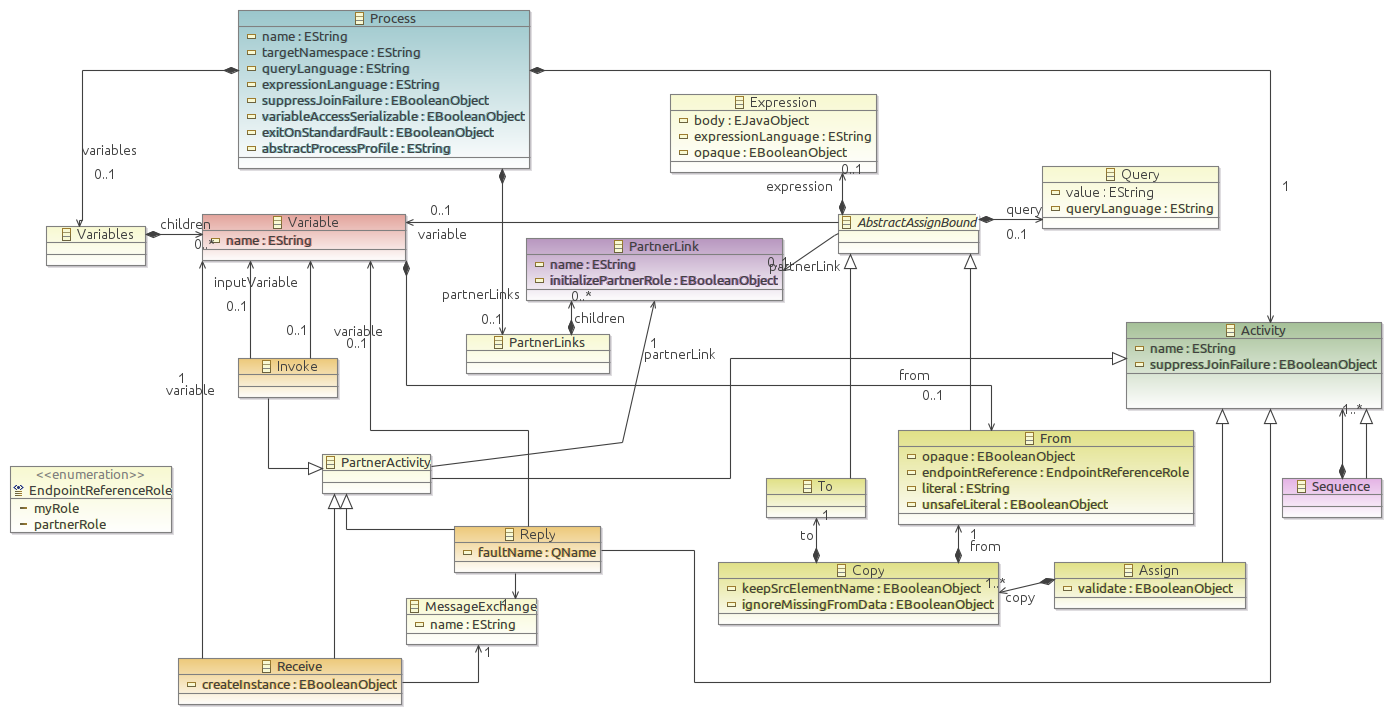
\includegraphics[scale=0.67,angle=90]{pictures/SubSetBpel2.png}
    \caption{The BPEL subset in its ecore model representation}
    \label{fig:SubSetBPEL}
  \end{center}
\end{figure} 

\subsubsection{The meta-model for the BPEL subset}
\label{Sec:DesignBpelSubset}
To permit the parameterization of the BPEL process input model, we need a meta-model describing our subset. The Eclipse Modeling Framework (see Section \ref{EMF}) provides a meta-model written in ecore for the whole BPEL language; we use only the subset elements of this ecore meta-model.
\subsubsection{The BPEL workflow pattern to focus on}
\label{sec:DesignBPELPattern}
The BPEL language with its wide range of activities and operation, gives the possibility to orchestrate many kind of workflow patterns among the participant services. We concentrate our attention on a process having the following participants:
\begin{itemize}
 \item one partner link representing a client
 \item one partner link describing a web-service
\end{itemize}
and on a simple workflow pattern that concerns the activities shown in Figure: \ref{fig:BPELWorkflowPattern}\footnote{This Figure has been realized using the BPEL designer facilities of Eclipse. Yet not a standard, as the Oasis consortium has not released a graphical standard, many vendors provide very similar graphical notations}. The pattern shown in the Figure includes the following steps:
\begin{enumerate}
 \item the process waits for a client to connect and provide an input
\item reception of the input and its assignation to a variable to forward to the web-service.
\item web-service invocation
\item reception of the web-service's reply and assignation to a variable to be forwarded back to the client
\item final response sent back to the client
\end{enumerate}


\begin{figure}
  \begin{center}
    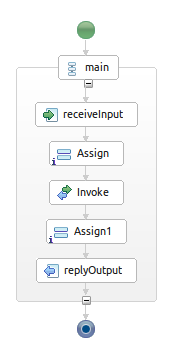
\includegraphics[scale=0.8]{pictures/BPELSimpleProcess.png}
    \caption{The BPEL workflow pattern we focus on}
    \label{fig:BPELWorkflowPattern}
  \end{center}
\end{figure} 

%///////////////////////////////////////////////////////////////
\subsection{Transformation Strategy}
\label{sec:TransformationStrategy}
As a direct transformation from BPEL constructs in Java concepts is neither feasible nor advisable, we have to provide a general strategy tackling single or groups of BPEL activities and creating Java counterparts. The following sections describe the single components of this strategy.

\subsubsection{The input files we work on}
\label{sec:inputFiles}
In a simple BPEL process there are two kind of files containing data valuable for our transformation: the BPEL process description files and the WSDL files to describe the services the process is orchestrating.
The BPEL process files contain: 
\begin{itemize}
 \item the definition of the partner links
 \item the variables used by the process to store or forward information
 \item the orchestration logic.
\end{itemize}
The WSDL files contain, in each file: 
\begin{itemize}
 \item the definition of a service
 \item the basic types used by the service's operations (\verb|<portType>|)
 \item the messages that contain elements of the basic types
 \item the service's definition including its name, server IP and port address. 
 \item the binding definition, which tells how a client could access the service (e.g. using the SOAP protocol)
\end{itemize}

\subsubsection{Translating the WSDL messages structure}
\label{sec:WSDLMEssagesStructure}
A very important feature of our transformation is to be able to generate a data definition specular to the one contained in the WSDL messages definition. WSDL messages can contain, for example, many elements of other types, and these types are, recursively, defined in the WSDL file. An example of the usage of the wsimport routine is shown in Figure \ref{fig:wsimport} where a BPEL message (SimpleProcessRequestMessage) definition is translated in the correspondent Java data structure (SimpleProcessRequest.java).
Instead of taking over the whole task of recreating the messages in Java, we reuse one of the already existing routines to generate the messages structure contained in a WSDL file in Java classes. From the many available, we picked the \textit{wsimport} routine \cite{wsimport}, freely available from the Oracle website. Of the wsimport features, we are interested in the one that translates the xml-written messages types described in the WSDL file in ready to use (and documented) Java classes. The classes and the attributes keep the names used in the WSDL file, making them aligned with the names found in the BPEL process description.
This tool proved very useful as we could make use of a reliable and tested solution, and at the same time concentrate the extra time gained on the transformation's logic. 

\begin{figure}
  \begin{center}
    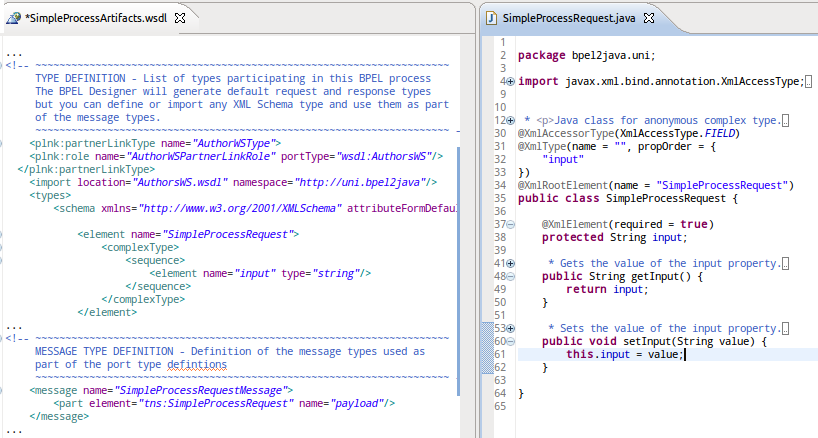
\includegraphics[scale=0.57]{pictures/wsImport.png}
    \caption{An example of how the wsimport routine works on translating a WSDL message (SimpleProcessRequestMessage) type information in the correspondent Java data structure (SimpleProcessRequest.java)}
    \label{fig:wsimport}
  \end{center}
\end{figure} 

\subsubsection{Mimic the BPEL workflow logic}
\label{mimicBPELLogic}
The BPEL orchestration logic is contained in a well defined section of a BPEL file. In the case of our BPEL subset, the logic workflow is all included in the \textit{sequence} activity. When generating the Java code, we make sure that the instructions included in the \textit{sequence} all end up in a Java class called after the process' name (we refer to it as the \textbf{Process class}). This class has a method \textit{runWorkflow()} that takes care of creating the instances of the PartnerLinks involved in the process and mimics the BPEL workflow activities.  
This allows us to decouple the logic from the data storage and management. Moreover, this separation makes room for future development regarding, among others, the enlargement of the BPEL activities subset. For example, if the \textit{pick} activity will, one day, be incorporated, the process class is the only class where changes will take place.

\subsubsection{The External Resources: Partner Links}
\label{sec:extrenalResources}
For what it concerns the external resources, namely, the web service orchestrated by the BPEL process, they are all defined in the BPEL \textit{partnerLink} (we will often refer to it as PL) construct. For each of the partnerLinks we create a class containing the \textit{variables} (Java attributes) and the \textit{portTypes} (Java methods) which are specular to the operations offered by the real service.
One thing to note is that we make a difference between the Client PL and the other PLs defining the rest of the services. The client PL is the one that usually initiates a BPEL workflow with a request message, while the other PLs are representing services that will be called from inside the BPEL workflow. For testing purposes, we create the client partnerLink class in order to have some more freedom-of-intervention in the generated code.

\begin{figure}
  \begin{center}
    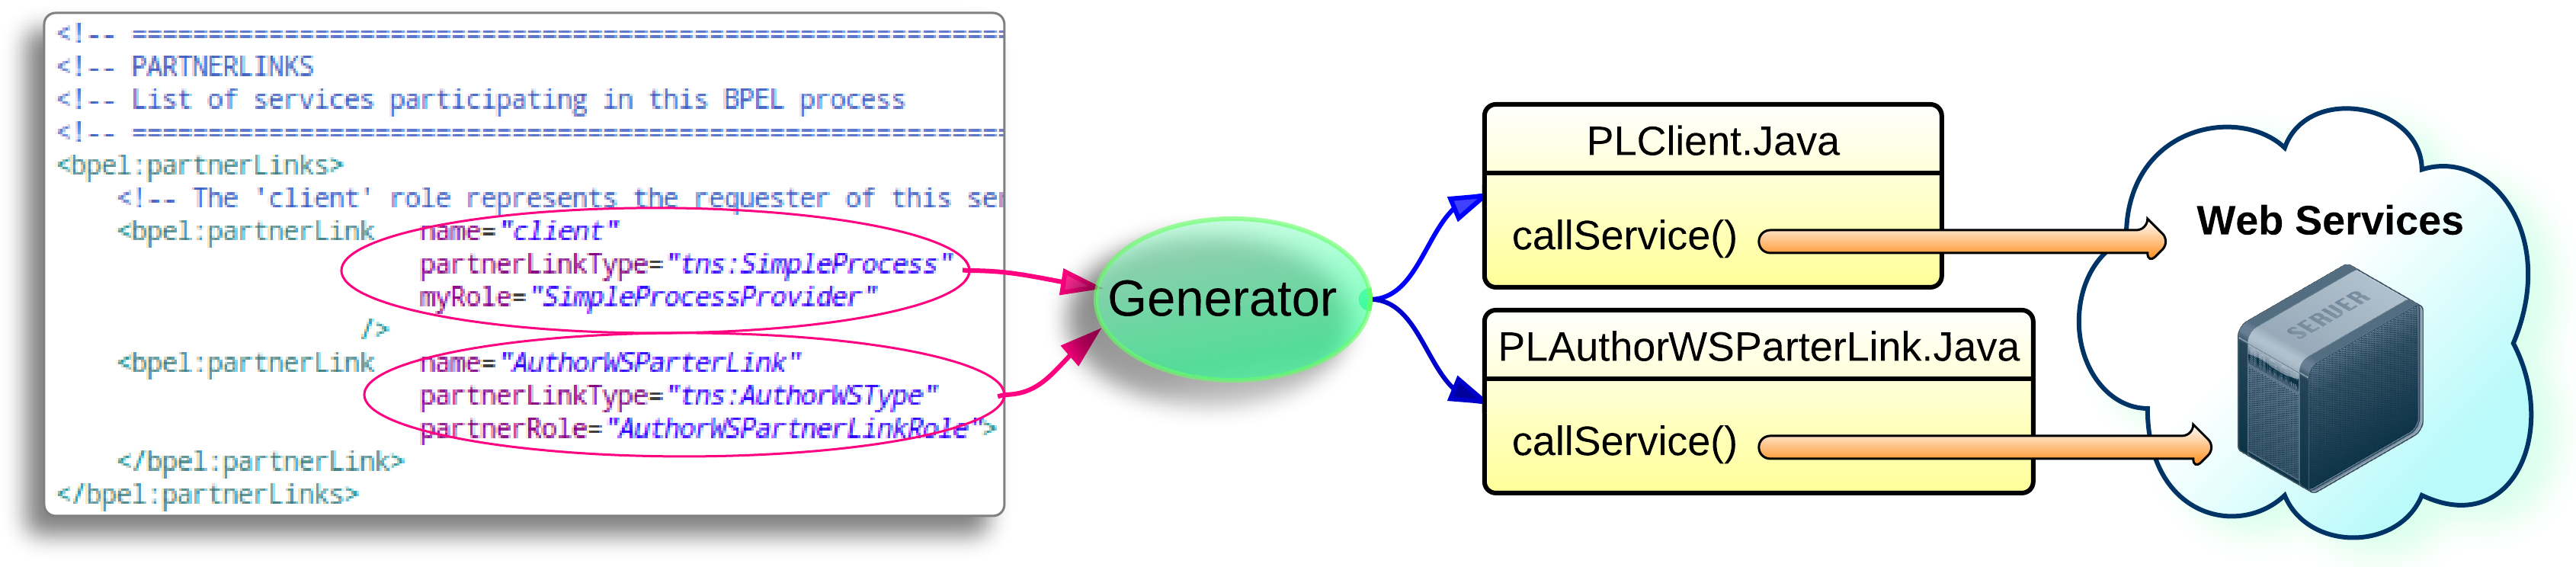
\includegraphics[scale=0.9]{pictures/PLTranslation.png}
    \caption{From the PartnerLinks listed in the BPEL process, our strategy is to create specular Java classes containing the code to call the web-services}
    \label{fig:PLTranslation}
  \end{center}
\end{figure} 


\subsubsection{Decoupling generated code from resources access}
\label{sec:decouplingPL}
The \textit{partnerLinks} (PL) represent a model of real world services, deployed on some servers. These services might present different binding characteristics, described in the WSDL file. Our strategy is to avoid to generate directly in the Java application the calls to these services. From the Partner links classes we create stub methods, mimicing the services' operation names (the names end with a "stub" suffix), that have the only task of forwarding the calls to the real service. 
This is also done in order to leave room to the developer in case the service calls have to be made in a special way, or the WSDL files are not accessible. The developer can just intervene in the body of the stub methods and write the calls to the specific service's operation.

\subsubsection{Summary of the transformation strategies}
\label{transfStrategySummary}
Table \ref{tab:transStrategies} briefly summarizes, for an easier consultation, the transformation strategies we have selected. 
%%%%%%%    Table %%%%%%%%%%%%%%%%%%%%%%%%%%%%%%%%%%%%%%%%%%%%%%
\begin{table}
\caption{The main BPEL-to-Java transformation strategies we adopt}
\label{tab:transStrategies}
\begin{center}
\begin{tabular}{p{5cm} p{9,8cm}}
						\toprule
						\addlinespace[0.2cm]
\textbf{Concept} 		& \textbf{Transformation strategy} 	\\ 
						\cmidrule(l){1-2}
The input files to work on 	
				& taken into consideration the BPEL process descriptor file and WSDL web-service descriptor 			 			\\[0,5cm]
WSDL messages structure 	
				&  usage of the wsimport ORACLE routine to create, from the WSDL messages, the Java equivalent data structure  			\\[0,5cm]
Mimic the BPEL workflow logic 	
				& the \textit{process} class contains the logic of the BPEL process. The \textit{runWorkflow()} method creates the PL instances and mimics the BPEL workflow activities  			\\[0,5cm]
The External Resources: Partner Links 		
				&  there are created a class representing each of the partner links involved. A special client PL is also created with extra freedom-of-intervention, in order to better test the application	\\[0,5cm]
Decoupling generated code from resources access 
				& to represent the real service's operations, stub methods are created in the partnerLinks classes. They allow the developer to directly write the code to invoke the specific service's operation
				\\[0,5cm]
\addlinespace[0.2cm]
						\bottomrule
\end{tabular}
\end{center}
\end{table}
%%%%%%%%%%%%%%%%%%%%%%%%%%%%%%%%%%%%%%%%%%%%%%%%%%%%%%%%%%%%%%
\subsection{The Architectural of the Java Application}
\label{sec:JavaArchitecStruct}
Before starting the transformation, we should have a rough idea of the architecture that the Java generated application should comply with.
As our transformation deals with a small subset of the whole BPEL language, the correspondent Java application architecture does not seem to need, yet now, a strictly defined model. This happens because we do not want to force an architectural style that might restrict future expansions of the BPEL elements' subset.
Eventually, both for the reasons said above and a time wise concern, our strategy in this case is to keep the Java application's design as simple as possible, without creating inheritances or particular abstraction layers; the focus will then be on the transformation and on the generation of a runnable Java process.

\subsection{Instances of the generated Java application}
\label{sec:JavaAppRunnable}
In BPEL, to create an instance of a workflow, there is at least one special attribute called \textit{createInstance = yes/no} that has to be set to "yes" inside a \textit{receive} or \textit{pick} activity \cite{BPEL-oasis}. In the Java generated Java application, to obtain a similar behaviour, one should create an instance of the process class (the one containing the workflow logic). Once an instance is created, the method \textit{runWorkflow()} has to be invoked. This method takes care of creating all the instances of the partnerLink classes, and make the needed calls to carry out the workflow.
Having the whole BPEL process' sequence of steps in one method might be quite cumbersome, especially in the case where the workflow pattern has several activities and conditions. In our case, though, the workflow complexity problem does not arise because of two reasons: the usage of a subset of BPEL instruction and, most importantly, the workflow pattern has been fixed a-priori (see Section \ref{sec:DesignBPELPattern}). 

\subsection{Java templates and the dynamic BPEL information}
\label{TemplatesDynamicInfos}
The parameterized information taken from the BPEL and WSDL models are present in many parts of the Java templates. The names of attributes, operations, variables and messages all correspond to the original names from the input model. 
We also tried to keep the names of the files synchronized with the names of the BPEL elements. For example, while creating the partnerLink stub classes, the classes keep the same name as the partnerLink, adding only a "PL" prefix. 
The generator also have to be able to deal with a dynamic number of BPEL elements. Messages, variables, types and  partnerLinks can be present in any number in the input model; the generator detects them and create the correspondent Java concepts/classes.

Concerning the workflow logic, as we have fixed the BPEL pattern we work on, we actually know how many and which BPEL activities to expect. From any of these activities the generator selects the information needed to translate each of them in Java method calls. 
For example a \textit{receive} activity that in BPEL is coded as:

\begin{workflow-code}{A receive activity in BPEL}{lis:receiveBPEL}
<bpel:receive name="receiveInput" partnerLink="client"
                 portType="tns:SimpleProcess"
                 operation="process" variable="input"
                 createInstance="yes"/>
\end{workflow-code}

In Java we transform the \textit{receive} activity (as shown in Listing \ref{lis:receiveInJava}) extracting the following parts: the name of the partnerLink owner of the operation ("client") from which we understand the partnerLink instance class we have to use ("myPLClient"), the name of the partnerLink instance class' method ("receiveInput()") and the name of the variable ("input") that is used in the body of the receiveInput() method to set the correspondent private variable. 

\begin{java-code}{A receive activity translated in Java}{lis:receiveInJava}
// Emulate the Receive activity		
		myPLClient.receiveInput();	
\end{java-code}

Eventually, the translation of the BPEL workflow in Java will all be contained in the \textit{runWorkflow()} method of the process class. The body of the runWorkflow method contains the code to control that the input pattern complies with our pattern. In addition, it contains the Java calls resulting from the translation of the single parts of the patter (receive, assign, invoke, assign and reply).

\subsection{The developer's intervention}
\label{sec:developerIntervention}
As already described in the introduction, we attempt a t carry out a transformation with the least developer's intervention as possible.
Theoretically, having at complete disposal the BPEL input model and the WSDL descriptors files, there should be almost no developer's intervention at all. Though, as described in Section \ref{sec:issues}, some problems arisen with the technology we decided to use made the manual intervention necessary in some cases:
\begin{itemize}
 \item insertion of the types of the BPEL variables
 \item association between partnerLink-to-variable during an assign
\end{itemize}
We will describe these cases in detail later in the report.

\subsubsection{How to Control the type of Workflow Pattern}
Concerning the control of the type for the BPEL pattern input by the user, in our  case we develop the control structure directly inside the generator. That means we check at the beginning that the given BPEL input model complies with our previously specified pattern.
If other BPEL workflow patterns will be include in the future, it will be easy to create a pattern control module, which recognizes the input pattern and applies the right transformation on it.